% -*- coding: utf-8 -*-
%%\mainmatter
\cleardoublepage
\chapter{Método de trabajo}
\thispagestyle{fancy}
%%\setcounter{page}{22}

\drop{E}{n} este capítulo se describe la metodología utilizada durante el desarrollo
de FreeStation. En el Capítulo 6 se describen las iteraciones de este
desarrollo, junto a la complejidad y resultados de cada una.

\section{\uppercase{Metodología de trabajo y desarrollo}}

El marco usado para estructurar y planificar el proceso del desarrollo del
software distribuido seguirá las herramientas y modelos establecidos en la
metodología \emph{Extreme Programming}\cite{Bec01} donde dicho enfoque permitirá
de forma ágil experimentar una adaptabilidad sobre los requisitos naturales del
sistema.

Cualquier cambio necesario en algún punto de vida del proyecto será más
realista y controlable con esta metodología
basada en paradigmas de simplicidad (refactorización de código iterativa,
con autodocumentación del código),
comunicación (pruebas unitarias de la funcionalidad), retroalimentación
(valoración de resultados de salida en cada iteración).

Puesto que la arquitectura cumple con una estructura modular e incremental, el
trabajo pudo ser dividido en iteraciones, valorando el resultado final en cada
entrega.

\begin{figure}[ht]
    \begin{center}
        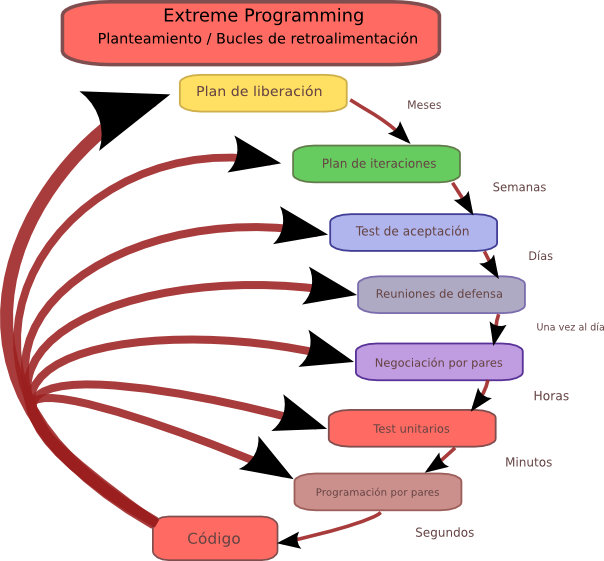
\includegraphics[width=400px]{src/img/extreme-programing-graph.png}
        \caption[Ciclo de Extreme Programming] {Ciclo de Extreme Programming}
    \end{center}
\end{figure}

\newpage
Este enfoque permite una mayor adaptabilidad con principales valores como
comunicación, sencillez y retroalimentación\cite{Bec00}.

En el proceso se realizarán pruebas, que permitirá afianzar el trabajo y tener
una mejor respuesta a introducción de fallos inadvertidos.

\section{\uppercase{Requisitos funcionales}}

Para establece unos requisitos funcionales, por un lado es necesario efectuar un
estudio previo de la situación actual.
Esto implica el análisis de otros sistemas con funcionalidades similares, buscar
ventajas e inconvenientes de cada uno de ellos y determinar a partir de ahí las
funcionalidades deseables en nuestro sistema.

Por otro lado: definir un objetivo fijo, establecer los límites de definición
del proyecto y evaluar y definir las funcionalidades del sistema.

Los usuarios finales demandan una atención al tiempo de respuesta final del
proceso solicitado. La actualización del software obtenido en una red de
distribución debe minimizarse al máximo\cite{Bau10} y requerir de una
atención mínima por sus supervisores para una gran red.

Esto requiere a su vez de una interfaz modularizable por la parte final de los
usuarios, donde con simples acciones e intuitivas se permita realizar las
acciones requeridas.

\section{\uppercase{Requisitos estructurales}}

El sistema debe contar con una estructura muy tolerante a fallos,
donde un simple error no comprometa al sistema e incluso se recupere del mismo
si fuera posible. En caso de no ser posible, este al menos debería contar
con un buen informe para los supervisores de la red, para que en cualquier
momento un problema sea identificado y reparado en el menor tiempo posible.

La demanda de software por los usuarios, debe ser realizada en imágenes
(ISO) personalizadas y parametrizadas para cada subsistema en un centro de
software distribuido. Estas imágenes deben ser regeneradas y actualizadas
cuando el sistema lo requiera o sus supervisores lo necesiten.

\section{\uppercase{Casos de prueba}}

La gestión de calidad de software dependerá de las transformaciones sufridas
en su distribución.
La seguridad y conformidad del despliegue software permitirán una alta
solución al problema donde los requisitos sea cumplidos sin ningún defecto.

Al encontrarse el sistema automatizado, el escenario de uso común de un
usuario estará plenamente abordado por el sistema permitiendo distribuir el
software ordenador por el usuario final sin ninguna complicación.

El rendimiento y la escalabilidad del sistema permitirán una amplia gama de
aplicaciones disponible convirtiendo al sistema en un catálogo completo
personalizado con la precisión establecida.

Partiendo de un conjunto de funcionalidades en forma de requisitos es posible
especificar un diseño global del sistema. Este define su estructura,
componentes, módulos y datos del sistema.

\section{\uppercase{Medios utilizados}}

Los medios requeridos para el desarrollo tienen en cuenta la utilización de la
infraestructura de repositorios, servidores, clientes, etc, que serán usados
en la red de la Universidad de Castilla-La Mancha (UCLM) en colaboración
con los equipos de grupo de
investigación ORETO\footnote{ORETO:
\url{http://oreto.esi.uclm.es}\label{ftn:Oreto}}.

Se utilizara repositorios de control de versiones GIT\footnote{GIT:
\url{http://git-scm.com}\label{ftn:GIT}} para la administración del desarrollo
del código utilizado.

El sistema cliente y servidores funcionarán con sockets escritos mayormente en
python, donde la comunicación mediante datos crudos, datos estandarizados
(\acs{XML}\label{acro:XML}) o invocaciones remotas, definirán actuaciones del
sistema y sus posibles consecuencias. Posteriormente se utilizarán 
frameworks de objetos distribuidos para envío y recepción de datos remotos.

La supervisión y monitorización\cite{Mar11} sera realizada tanto de forma
interna por el sistemas como con la ayuda de aplicaciones terceras que
informen a este de posibles errores en el mismo o elementos de aviso para sus
administradores.

La documentación general del sistema será especificada y parametrizada para
clientes y servidores con el fin de obtener una gran modularidad y
adaptabilidad del sistema ante requisitos que puedan surgir en la posible vida
del proyecto en un centro de distribución software.

\newpage

\subsection{Herramientas}

A continuación se enumeran y describen los recursos hardware y software
utilizados durante el desarrollo, indicando las versiones específicas
empleadas en la construcción de la versión de FreeStation adjunta en el CD que
acompaña a la presente memoria.

El software y hardware durante el desarrollo ha seguido dichas especificaciones
por lo que se recomienda realizar una configuración similar con el fin de
obtener los mismos resultados. Existe la posibilidad de utilizar versiones
superiores de software u otros componentes hardware.

No se aseguran la exactitud de los mismos resultados de ejecución, aunque el
software ha sido desarrollado de forma adaptativa para tratar de minimizar
el impacto de errores o fallos derivados de distintas configuraciones.

\subsection{Lenguajes}

Para la realización de FreeStation se han utilizado diversos lenguajes de
programación, que se listan a continuación:

\begin{itemize}
\item \textbf{\acs{PHP}\label{acro:PHP}}\footnote{PHP:
\url{http://php.net}\label{ftn:PHP}}:
es el lenguaje utilizado principalmente en el desarrollo del proyecto para la parte Frontend del modelo servidor web.
El proyecto ha sido implementado usando una versión compatible con
PHP 5.3.X.

PHP es un lenguaje creado en 1994 por Rasmus Lerdorf para entornos de
binarios \acs{CGI}\label{acro:CGI}.

Esta escrito en el lenguaje C y gracias a su simplicidad creció rápidamente en
popularidad hasta convertirse en el lenguaje con mayor cuota de mercado de
creación para webs.

\item \textbf{Python}\footnote{Python: \url{python.org}\label{ftn:Python}}:
es el lenguaje utilizado para realizar scripting y la parte Backend del modelo servidor y modelo cliente. La versión
adjunta en el CD está compilada con soporte para Python 2.7.

Python es un lenguaje creado en 1989 por Guido van Rossum con el principal
objetivo de realizar programas legibles y de sintaxis clara. Es un lenguaje
para prototipado rápido y aplicaciones críticas con mucho potencial
matemático.

\end{itemize}

\newpage

\subsection{Hardware}
\label{sec:harware}
La mayor parte del desarrollo de FreeStation se ha realizado usando varios nodos
cliente y servidor.

Las especificaciones de hardware no son elevadas para uso de nodos clientes,
aunque la especificación para un nodo servidor, viene determinada por el número
de clientes que se conecten y el tráfico simultáneo en pico que deba soportar el
nodo servidor.

Las características más notorias para la aplicación son la concurrencia de CPUs
y la capacidad de memoria. La capacidad de disco duro, operaciones de
entrada/salida u otros factores son importantes, pero quedan establecidos según
configuraciones particulares que se demanden.

Para los nodos clientes se han usado 4 portátiles y un ordenador de sobremesa:

\begin{itemize}
\item Acer Aspire Ethos 5943G (laptop): 4 GB RAM, 4 núcleos.
\item Acer Aspire One (netbook): 2 GB RAM, 2 núcleos.
\item Compaq Presario C700: 1 GB RAM, 1 núcleo.
\item HP 620: 4 GB RAM, 2 núcleos.
\item Sobremesa: 4 GB RAM, 4 núcleos.
\end{itemize}

Para el nodo servidores se han usado varias máquinas virtualizadas:

\begin{itemize}

\item Bajo virtualización OpenVZ\footnote{OpenVZ:
\url{http://openvz.org}\label{ftn:OpenVZ}}:
512 MB ram, 2 núcleos, para entorno de desarrollo y pruebas y de bajas características durante el desarrollo.

\item Bajo virtualización VMWare\footnote{VMWare:
\url{http://vmware.com}\label{ftn:VMWARE}}:
como entorno de producción bajo de 4 cores y 8 GB RAM.

\end{itemize}

\subsection{Software}

A continuación se lista todas las herramientas y bibliotecas software utilizadas
para el proyecto. Estas herramientas justifican la importancia crucial para un
ámbito de desarrollo, con el fin de ofrecer unas condiciones similares para este
proyecto de fin de carrera. Se describen por subapartados y tecnologías
específicas.

\subsubsection{Sistemas operativos}

Las preferencias se basaron en sistemas operativos basados en software libre y
de amplia distribución. 

Se han usado los siguientes:

\begin{itemize}

\item \textbf{Ubuntu}\footnote{Ubuntu:
\url{http://ubuntu.com}\label{ftn:Ubuntu}}:
como sistema operativo principal se ha utilizado Ubuntu 11.10, 12.04 y 12.10
durante el desarrollo, siendo imprescindible ubuntu 12.10 para la versión
cliente. Se ha elegido por considerarse una de las distribuciones de
GNU/Linux más usadas y sencillas para desarrolladores y estar basada en 
Debian. La totalidad de aplicaciones de este proyecto han sido desarrollado
bajo este sistema operativo.

\item \textbf{CentOS}\footnote{CentOS:
\url{http://centos.org}\label{ftn:CentOS}}: como sistema operativo para
nodos servidores, basada en RedHat.

La versión utilizada ha sido la rama 5, con actualizaciones hasta
la versión 5.8. La elección fue por la estabilidad y conocimiento previo de
la distribución para servidores.
\end{itemize}

\newpage

\subsubsection{Entornos de desarrollo}

La totalidad del proyecto ha sido desarrollada con \acs{IDE}\label{acro:IDE}s
que permitieran un rápido desarrollo. Los más utilizados han sido:

\begin{itemize}

\item \textbf{Eclipse}\footnote{Eclipse:
\url{http://eclise.org}\label{ftn:Eclipse}}: se utilizó la plataforma de
desarrollo Eclipse 3.7 y 3.8, junto al plugin desarrollo para PHP (PDT, PHP
Development Tools v 3.0) para el frontend web en PHP, el plugin PyDev v2.2 para el backend en Python y desarrollo en ICE,
y los plugins ShellEd 2.0 y TeXlipse 1.5 para scripts y documentación en
LaTeX.

\item \textbf{Geany}\footnote{Geany:
\url{http://geany.org}\label{ftn:Geany}}: es un editor de texto que usa GTK
con las características básicas para un entorno de desarrollo. Fue utilizado
para edición de archivos simples y configuraciones de forma rápida al ser
un editor rápido y ligero basado en un motor escrito en C.

La versión utilizada fue la 1.22 con el nombre en código ``Tavira''.
\end{itemize}

\subsubsection{Entorno de depuración y perfilado}

Para desarrollar un software depurado, que evite en la mayor medida fallos y
cuellos de botella, se utilizaran herramientas de depurado y perfilado como las
siguientes:

\begin{itemize}

\item \textbf{Xdebug}\footnote{Xdebug:
\url{http://xdebug.org}\label{ftn:XDebug}}: es el depurador y perfilador por
excelencia de PHP escrito por Derick Rethans. Tiene una gran variedad de parámetros de configuración, depuración remota, integración con muchos IDEs (Eclipse,
Netbeans, etc)

\item \textbf{KCacheGrind}\footnote{KCacheGrind:
\url{http://kcachegrind.sourceforge.net/html/Home.html}\label{ftn:KCacheGrind}}:
es un programa de escritorio (en especial para diseñado para KDE, pero compatible para GNOME) escrito para visualizar los
archivos de depuración generados por xdebug. Es un frontend de
Callgrind\footnote{Callgrind:
\url{http://valgrind.org/docs/manual/cl-manual.html}\label{ftn:Callgrind}},
que a su vez usa en tiempo de ejecución al framework de Valgrind para simulación de caches y generación de las llamadas gráficas.

\newpage
\item \textbf{Webgrind}\footnote{Webgrind:
\url{https://code.google.com/p/webgrind/}\label{ftn:Webgrind}}: es un
perfilador gráfico de código PHP vía web escrito en PHP por Joakim Nygård y Jacob Oettinger.
Tiene como dependencia Xdebug ya que es en realidad un wrapper web no
completo de las funciones de KCacheGrind como reemplazo de
frontend web de xdebug.

Se ha utilizado para depurar código, optimización de cuellos de botella y mejoras de rendimiento.

\end{itemize}

\subsubsection{Entorno de pruebas unitarias}

\begin{itemize}

\item \textbf{PHPUnit}: es un entorno para realizar pruebas unitarias en
el lenguaje de programación PHP creado por Sebastian Bergmann.
Se ha utilizado para detectar los errores en el código durante el desarrollo
y evitar la introducción de nuevos en partes probadas.

\item \textbf{PyUnit\footnote{PyUnit:
\url{http://pyunit.sourceforge.net}\label{ftn:PyUnit}}/unittest\footnote{Unittest\url{http://docs.python.org/library/unittest.html}\label{ftn:Unittest}}
}: es un estándar
probado como framework simple y elegante de pruebas unitarias en
programas Python (módulo
unittest).

Se ha utilizado para realizar una pequeña batería de pruebas unitarias en
algunas de las clases y código más crítico del proyecto, en particular la
parte backend de cliente y servidor escrita en Python.

\end{itemize}

\subsubsection{\uppercase{Otras aplicaciones}}

\begin{itemize}

\item \textbf{MySQL}\footnote{Mysql:
\url{https://mysql.com}\label{ftn:MySQL}}: es el sistema de gestión de base de
datos relacional (\acs{RDBMS}\label{acro:RDBMS}) más usado en el mundo que es
ejecutado en modo servidor proporcionando un acceso multi-usuario a un gran número de bases
de datos.

Se ha utilizado como servidor de base de datos en
la capa de persistencia de backend y frontend servidor.

La versión utilizada ha sido MySQL 5.1.
\end{itemize}

\newpage

\subsubsection{\uppercase{Documentación y gráficos}}

\begin{itemize}
\item \textbf{Make}\footnote{make:
\url{https://gnu.org/software/make/}\label{ftn:Make}}:
Herramienta que se ha utilizado para el proceso de compilación de los
archivos fuente del proyecto (en mayoría fuentes
relacionadas con la documentación, ya que archivos fuente en php y python
no requerían de esta utilidad). La versión que se ha utilizado es la 3.81.

\item \textbf{Bash}\footnote{bash:
\url{https://www.gnu.org/software/bash/manual/bashref.html}\label{ftn:Bash}}:
para creación de scripts de compilación, generación de documentación y otras utilidades relacionadas en el proyecto. La versión
utilizada ha sido 4.2.10.

\item \textbf{\LaTeX}\footnote{\LaTeX:
\url{http://latex-project.org}\label{ftn:latex}}: el framework de
composición de documentos libres y profesionales que se ha usado para generar este proyecto de fin de carrera.
Se ha utilizado la versión 3.1415926-1.40.10-2.2 (TeX Live 2009).

El código fuente del proyecto y documentación están disponibles en fuentes para este programa
bajo licencia \acs{FDL}\label{acro:FDL}.

\item \textbf{LibreOffice Draw}\footnote{LibreOffice Draw:
\url{http://es.libreoffice.org/caracteristicas/draw/}\label{ftn:Draw}}:
herramienta de dibujo vectorial utilizada para la generación de figuras e imágenes para
la documentación, en su versión 3.4.

\item \textbf{LibreOffice Calc}\footnote{LibreOffice Calc:
\url{http://es.libreoffice.org/caracteristicas/calc/}\label{ftn:Calc}}:
herramienta de creación y manipulación de hojas
cálculo, utilizada para la generación de gráficos estadísticos de la
documentación. Se ha aplicado la
versión 3.4.

\item \textbf{The Gimp}\footnote{The Gimp:
\url{http://gimp.org}\label{ftn:Gimp}}: es una potente
herramienta de manipulación de gráficos de software libre utilizada para
la documentación y generación de gráficos para demostraciones.

Se ha utilizado la versión 2.6.11.

\item \textbf{Inkscape}\footnote{Inkscape:
\url{http://inkscape.org}\label{ftn:Inkscape}}: es un editor de
Gráficos Vectoriales, similar al Adobe Illustrator,
que busca ser compatible con SVG, de código abierto, sensible y
extendible.

Se ha usado para la creación de diagramas y vectorizado de
aplicaciones.

\item \textbf{MySQL Worbench}\footnote{MySQL Worbench:
\url{www.mysql.com/products/workbench/}\label{ftn:workbench}}:MySQL
Workbench es una herramienta visual unificada para arquitecturas de bases
de datos y desarrolladores.

Permite un modelo de datos basado en el desarrollo SQL de datos en crudo y
un conjunto de herramientas comprehensivas para la administración.

Se utilizo la versión 5.1 para el modelado del diagrama E/R del esquema de
base de datos utilizado en la capa de persistencia de mysql.

\item \textbf{Gnome Dia}\footnote{Gnome Dia:
\url{https://live.gnome.org/Dia}\label{ftn:gnomedia}}: es una herramienta
de dibujo para diagramas y casos de uso.

Genera todo tipo de diagramas, se ha utilizado para desarrollar el esquemas
de clases.

Se ha utilizado la versión 0.97.1.

\end{itemize}

\subsection{\uppercase{Bibliotecas, plataformas y frameworks}}

\subsubsection{GTK}
\label{sec:GTK}
\textbf{\acs{GTK+}\label{acro:GTK+} o The GIMP Toolkit}\footnote{GTK:
\url{http://gtk.org}\label{ftn:Gtk}}: es un conjunto de bibliotecas
multiplataforma para desarrollar interfaces gráficas de usuario
(\acs{GUI}\label{acro:GUI}).

Las principales ventajas de GTK+ son:

\begin{itemize}
  \item Activamente desarrollado y mantenido con una comunidad fuerte.
  \item Ofrece extender la funcionalidad básica de widgets.
  \item Soporte de framework para internalización y accesibilidad.
  \item Software libre.
  \item Multiplataforma y portable.
\end{itemize}

La biblioteca que se
ha utilizado para la creación y la gestión de las interfaces gráficas del
proyecto.

En particular se ha usado su binding para Python, llamado PyGTK
y que en el desarrollo derivo
a la versión de PyObject

\newpage

\subsubsection{ZeroC ICE}
\label{sec:ZeroICE}
ZeroC \acs{ICE}\label{acro:CIE} (ZeroC Internet Communications Engine) es un
middleware muy adecuado para desplegar y desarrollar aplicaciones de
sistemas distribuidos.

El objetivo de éste es hacer que la invocación a objetos remotos sea vista
por parte del programador como si se tratase de una invocación a objetos
locales.

La forma de llevar a cabo esta enmascaración es mediante un proxy en la
parte del cliente que actúe de intermediario entre el cliente y el objeto
remoto al que se quiere invocar.

Y en la parte del servidor se necesita un esqueleto que traduzca los eventos
que se van produciendo en la red a las correspondientes invocaciones de los
métodos remotos.

Esta traducción es necesaria debido a que la comunicación entre el
cliente y servidor, no deja de ser una comunicación que sigue un protocolo
de red como \acs{TCP}\label{acro:TCP}, \acs{UDP}\label{acro:UDP}, etc.

Debido a que ZeroC ICE permite que el cliente y el servidor estén
implementados en distintos lenguajes de programación. El lenguaje para
definir la interfaz que debe de ser idéntica a ambas partes se define
mediante Slice: lenguaje de especificación de interfaces para ZeroC ICE.

Las razones principales para usar ICE fueron:

\begin{itemize}    
    \item Es una buena herramienta de trabajo para entornos que sean
    bastante heterogéneos, donde el cliente y servidor puede estar escritos
    en lenguajes de programación muy diferentes y ejecutarse sobre
    plataformas, sistemas operativos o arquitecturas muy variadas.

    \item Su fuerte radica en un gran soporte de tecnologías de red
    con interacciones a bajo nivel de red, enfoque en la lógica de las
    aplicaciones y portabilidad de entornos muy diversos.

    \item La abstracción de red para detalles como abrir conexiones de red,
    serializado y des-serializado de datos transmitidos por red,
    reintentos fallidos de conexión y muchos otros detalles más de
    bajo nivel que ayudan a simplificar la capa de red\cite{Fou05}.

    \item Soporta bindings con bastantes lenguajes de programación como:
    C++, .NET, Java, Python\cite{Val06}, Objective-C, Ruby, PHP, y
    ActionScript.
    
    \item Integra en su propia implementación seguridad, que hace sencillo de
    usarla en redes públicas inseguras.

    \item La curva de aprendizaje\cite{Hen06} es sencilla y existe una gran
    infraestructura de aplicaciones técnicas que se ha desarrollado.
    
    \item Ice es software libre bajo licencia \acs{GPL}v2 y comercializado
    bajo la marca ZeroC\footnote{ZeroC: \url{http://zeroc.com/}
    \label{ftn:ZeroC}}.
\end{itemize}   

Por lo tanto, se consigue evitar complejidad innecesaria, haciendo la
plataforma fácil de usar y aprender. La implementación es eficiente
para red respecto a ancho de banda, uso de memoria y CPU.

\subsubsection{DBus}
\label{sec:DBus}

DBus\footnote{Dbus:\url{http://www.freedesktop.org/wiki/Software/dbus}
\label{ftn:DBus}} es una implementación de alto nivel de IPC similar a 
Corba o ICE para las aplicaciones de Gnome. Se base en un sistema de
mensajes enviados a un bus principal que permite a las aplicaciones enviar
mensajes para interactuar entre ellas.

Se ha utilizado por su integración con Gnome y eficiencia de implementación
con GNU/Linux probada en aplicaciones reales por un gran período de tiempo.

La principal ventaja es su utilidad para la detección de Hardware, como
nuevos dispositivos \acs{USB}\label{acro:USB}.

Su binding a python facilita la programación orientada a eventos y señales a
través de la intercepción de mensajes en el bus principal.

\newpage

\subsubsection{Gstreamer}
\label{sec:Gstreamer}

GStreamer\footnote{GStreamer:\url{http://gstreamer.freedesktop.org/}
\label{ftn:GStreamer}} es una biblioteca para construcción de gráficos o
interacción de componentes multimedia.

Soporta un gran rango para de componentes como reproducción de vídeo
OGG/Vorbis, streaming de audio/vídeo con efectos, editado y procesado de
vídeo no linear, etc.

Tiene una gran facilidad ofrecida por esta biblioteca es la capa de
abstracción a la hora utilizar códecs o formatos. La transparencia al programador permite
un desarrollo rápido enfocado al propósito real de la aplicación sin perder
eficiencia o versatilidad.

Es compatible con un gran rango de sistemas operativos, procesadores y
compiladores. Su desarrollo es muy activo y esta respaldado por grandes
empresas como
Collabora\footnote{Collabora:\url{http://collabora.com}
\label{ftn:Collabora}}, Fluendo\footnote{Fluendo:
\url{ http://fluendo.com} \label{ftn:Novacut}} y la práctica totalidad de
las distribuciones GNU/Linux lo incluyen en sus repositorios o de forma
nativa en el sistema.

El traspaso de datos es extremadamente liviano lo que permite repercutir en
una baja latencia y alto rendimiento.

Como característica adicional, posibilita la carga dinámica de
complementos, lo que hace posible la personalización de características
deseadas en cualquier momento.

Durante el desarrollo se uso la versión 0.10, pero posteriormente se cambio
a 0.11 (conocida como 1.0) por problemas de integración en el binding de
python. Ver iteraciones del capítulo 6 para mayor detalle.

%% Put a blank page for open next chapter on right page side
%\newpage
%\mbox{}
%\thispagestyle{empty}